\section{Specific Requirements} \label{sec:spec_requirements}

%More details on all aspects in Section 2 if they can be  useful for the development team

\subsection{External Interface Requirements} \label{external}

\subsubsection{User Interface} \label{user_interface}

In this section, we will present some mockup to make the reader better understand the idea of the structure of the final web page and application.

\myparagraph{Log In} 
\newline
The mockup in Figure \ref{fig:login} shows the login page of PowerEnJoy. Here, a VISITOR can log in into the application.

\vspace{70pt}

\begin{figure}[htbp]
\centering
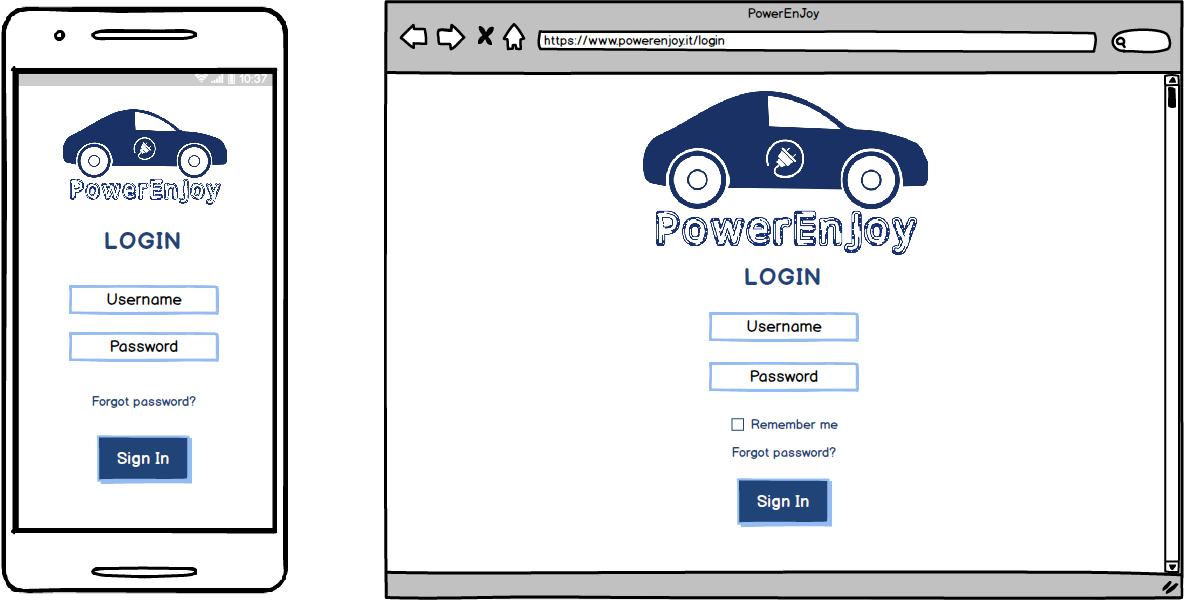
\includegraphics[width=\textwidth]{Images/Mockups/Login}
\caption{Log In Page mockup}
\label{fig:login}
\end{figure}
\clearpage

\myparagraph{Registration Form}
\newline
The mockup in Figure \ref{fig:registration} shows the registration form, where a VISITOR can sign up to access the service.

\vspace{80pt}

\begin{figure}[htbp]
\centering
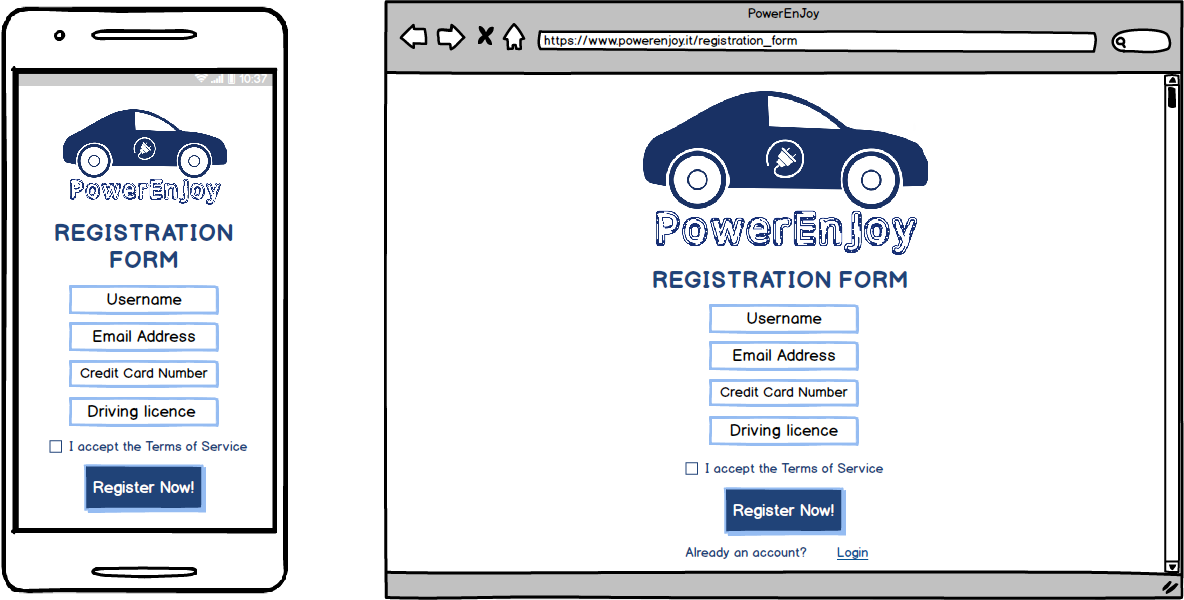
\includegraphics[width=\textwidth]{Images/Mockups/RegistrationForm}
\caption{Registration Form mockup}
\label{fig:registration}
\end{figure}
\clearpage

\myparagraph{Personal page}
\newline
The mockup in Figure \ref{fig:mypage} shows the personal page of a USER, from where he can update his data, such as, for example, the profile picture, the password and the payment information.

\vspace{80pt}

\begin{figure}[htbp]
\centering
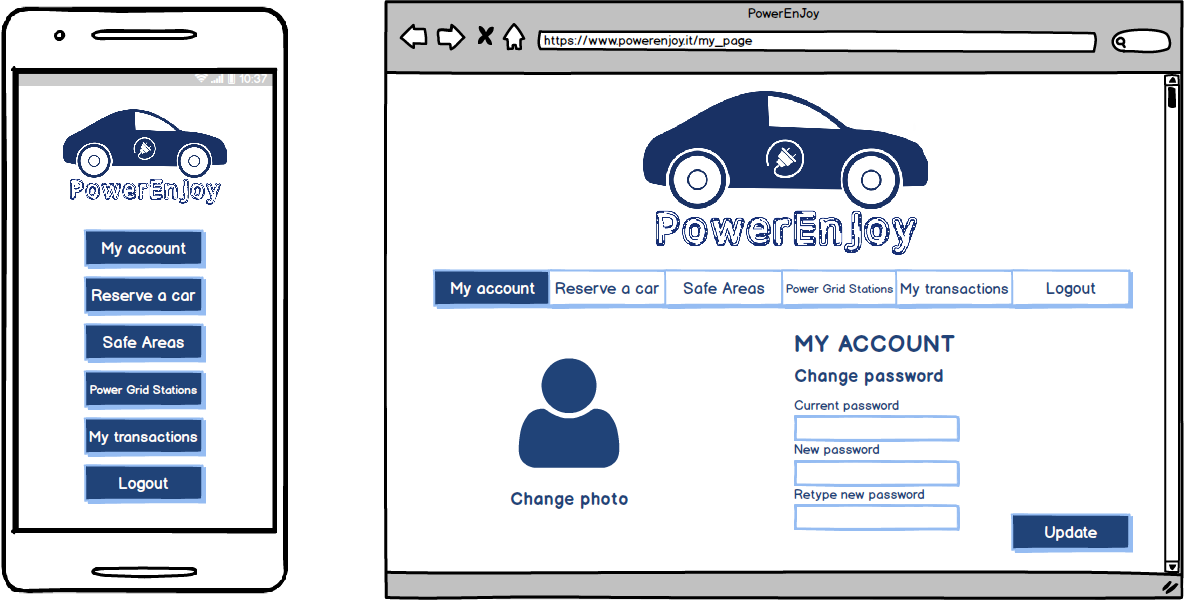
\includegraphics[width=\textwidth]{Images/Mockups/MyPage}
\caption{Personal Page mockup}
\label{fig:mypage}
\end{figure}
\clearpage

\myparagraph{Reservation page}
\newline
The mockup in Figure \ref{fig:reservation} shows the page from which a USER can reserve a car nearby him or near to a selected address for an hour.
He can also see how much time takes to get from the selected point to the car and its condition: level of charge and if it is plugged in a power grid station.

\vspace{80pt}

\begin{figure}[htbp]
\centering
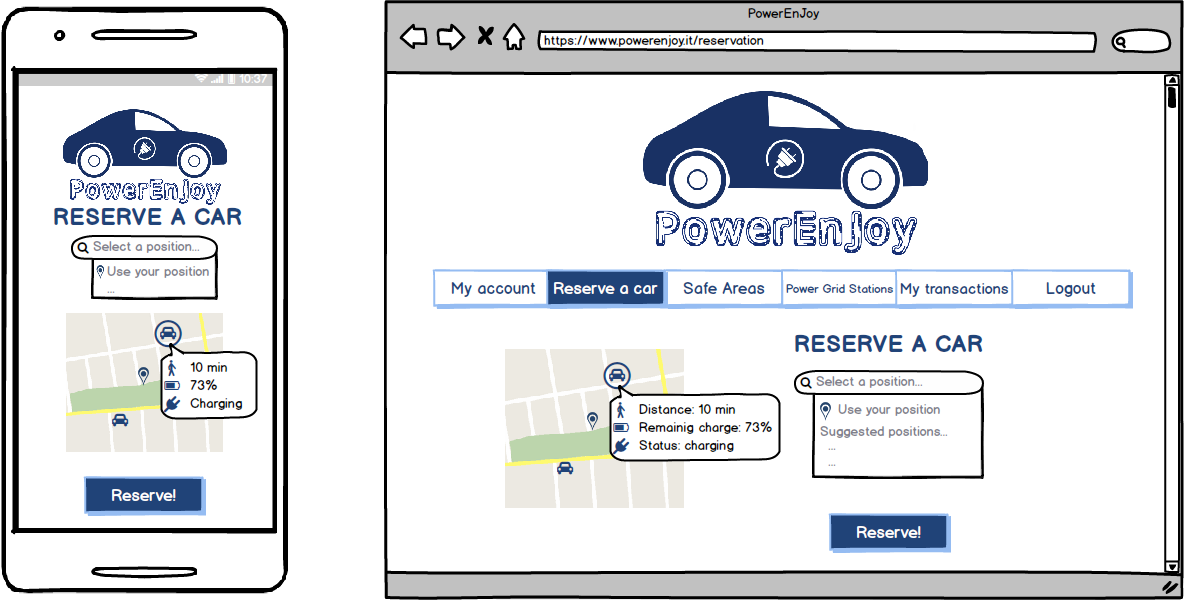
\includegraphics[width=\textwidth]{Images/Mockups/Reservation}
\caption{Reservation Page mockup}
\label{fig:reservation}
\end{figure}
\clearpage

Once the USER has made his reservation, the page and application will show him a 1 hour timer, as shown in Figure \ref{fig:timer}, in order to remind him how much time he has left to go and pick up the reserved car. In this time, the USER can decide to cancel his prenotation by clicking on the button "\textit{Cancel}". Only when the USER is nearby the car, he will be able to click the "\textit{I'm there}" button to unlock the reserved car.

\vspace{80pt}

\begin{figure}[htbp]
\centering
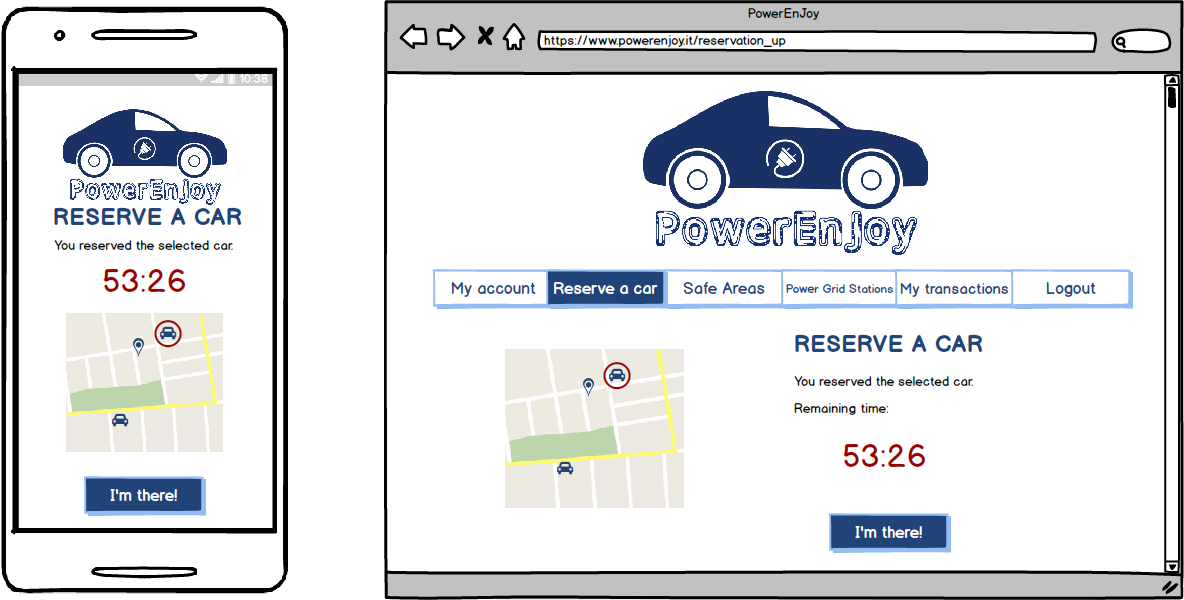
\includegraphics[width=\textwidth]{Images/Mockups/Timer}
\caption{Reservation Timer Page mockup}
\label{fig:timer}
\end{figure}
\clearpage

If the car is not picked up within an hour, the reservation expires: the USER is reminded that he has to pay a fee of 1 EUR, as shown in Figure \ref{fig:expired}.

\vspace{80pt}

\begin{figure}[htbp]
\centering
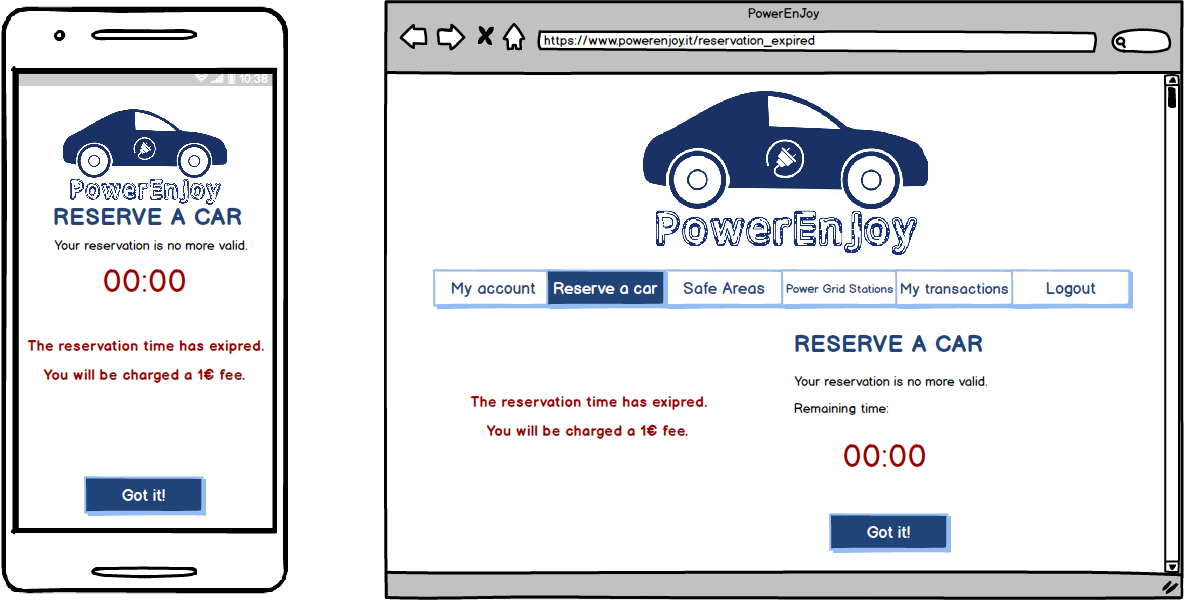
\includegraphics[width=\textwidth]{Images/Mockups/ReservationExpired}
\caption{Reservation Expired Page mockup}
\label{fig:expired}
\end{figure}
\clearpage

\myparagraph{Safe Areas page}
\newline
The mockup in Figure \ref{fig:safe} shows the page where the USER can visualize the safe areas around him or around a selected adderess.

\vspace{80pt}

\begin{figure}[htbp]
\centering
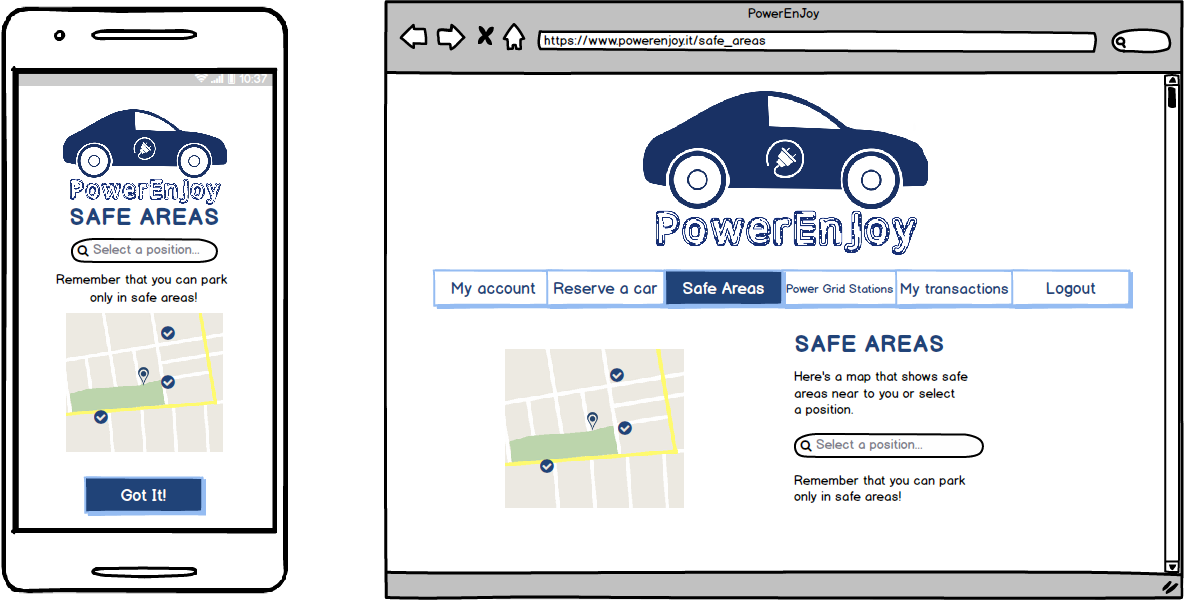
\includegraphics[width=\textwidth]{Images/Mockups/SafePlaces}
\caption{Safe Areas Page mockup}
\label{fig:safe}
\end{figure}
\clearpage

\myparagraph{Power Grid Stations page}
\newline
The mockup in Figure \ref{fig:power} shows the page where the USER can visualize the power grid stations around him or around a selected adderess.

\vspace{80pt}

\begin{figure}[htbp]
\centering
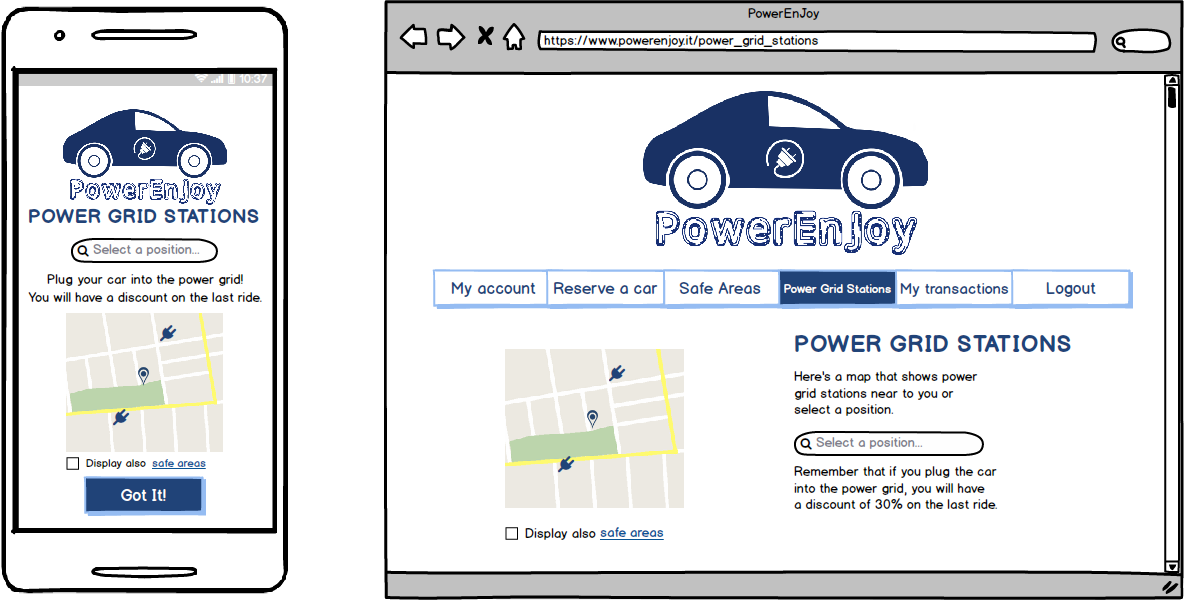
\includegraphics[width=\textwidth]{Images/Mockups/ChargePlaces}
\caption{Power Grid Station Page mockup}
\label{fig:power}
\end{figure}
\clearpage

\myparagraph{User's transactions page}
\newline
The mockup in Figure \ref{fig:transactions} shows the page where the USER can visualize his transactions and the relative details, such as the date of the ride, its duration and the discount or the increase on the fee to be payed.

\vspace{80pt}

\begin{figure}[htbp]
\centering
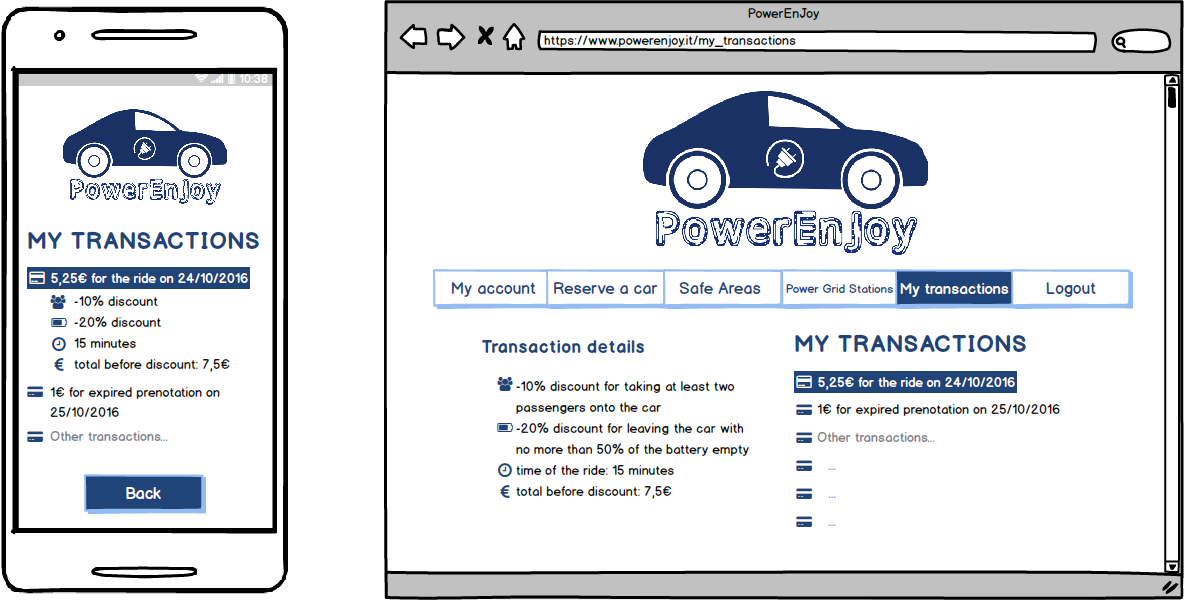
\includegraphics[width=\textwidth]{Images/Mockups/MyTransactions}
\caption{User's Transactions Page mockup}
\label{fig:transactions}
\end{figure}
\clearpage

\myparagraph{Car Screen}
\newline
The mockup in Figure \ref{fig:car} shows the car screen where useful information are visualized, for example the current level of charge, the duration of the rent and how much the USER has to pay before any discount or increase on the fee are applied.

\vspace{80pt}

\begin{figure}[htbp]
\centering
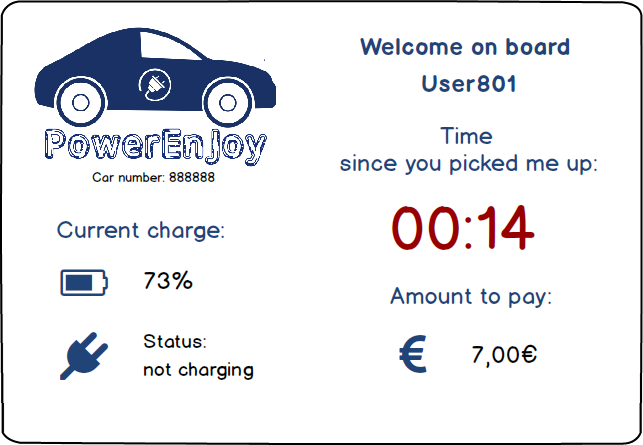
\includegraphics[width=\textwidth]{Images/Mockups/CarScreen}
\caption{Car Screen mockup}
\label{fig:car}
\end{figure}
\clearpage

\subsubsection{Hardware Interfaces} \label{hw_interfaces}
Device should be enabled with Internet and GPS receiver.

\subsubsection{Software Interfaces} \label{sw_interfaces}
The user's browser should be HTML5 compatible and the resolution should be at least 1280x720 for a satisfactory user experience.

%\subsubsection{Communication Interfaces} \label{comm_interfaces}

\subsection{Functional Requirements} \label{sec:funct_requirements}
In this section we explain all the functional requirements necessary to reach a specific goal. For each goal that was mentioned in the first section here we write its requirements.
\begin{itemize}
\item[\textbf{G1}]: 
\begin{itemize}
\item[--R1--] During the registration visitors can't choose an username already in use.
\item[--R2--] During the registration visitors can't choose an e-mail already in use.
\item[--R3--] During the registration visitors must insert valid credit card's information.
\item[--R4--] During the registration visitors must insert a valid driving license.
\item[--R5--] During the registration visitors must agree with the privacy conditions to use the system.
\end{itemize}

\item[\textbf{G2}]:
\begin{itemize}
\item[--R1--] The registration must be successfully completed.
\end{itemize}

\item[\textbf{G3}]:
\begin{itemize}
\item[--R1--] The user must be registered at the system.
\item[--R2--] In the log in form the user must insert the correct username.
\item[--R3--] In the log in form the user must insert the correct password.
\item[--R4--] If the visitor insert the wrong data, the system shows an error and return to the log in page.
\item[--R5--] If the user doesn't remember the password he can receive it trough a special command.
\end{itemize}

\item[\textbf{G4}]:
\begin{itemize}
\item[--R1--] The user must insert a valid address or give to the system his position.
\item[--R2--] All cars position must be knowed.
\item[--R3--] All cars are set as available or not.
\item[--R4--] The list of nearest cars is made trough calculate the distance between car and user's position.
\end{itemize}

\item[\textbf{G5}]:
\begin{itemize}
\item[--R1--] The user must be correctly logged in.
\item[--R2--] The user must select which car he wants.
\item[--R3--] The user must select only date and times valid for the reservation.
\end{itemize}

\item[\textbf{G6}]:
\begin{itemize}
\item[--R1--] The position of the user and the car must be the same.
\item[--R2--] The reservation must not be expired.
\item[--R3--] The system must recognize the correct car reserved by a specific user to unlock the correct one.
\end{itemize}

\item[\textbf{G7}]:
\begin{itemize}
\item[--R1--] The car's engine must ignites.
\item[--R2--] An amount of money per minute is set.
\item[--R3--] The final charge is based on the duration of the car use.
\end{itemize}

\item[\textbf{G8}]:
\begin{itemize}
\item[--R1--] There must be a display on the car that communicates with the system.
\item[--R2--] The charge is update every minute.
\end{itemize}

\item[\textbf{G9}]:
\begin{itemize}
\item[--R1--] It must be passed one hour from the registration.
\item[--R2--] Is applyed a fee of 1 euro to the user involved.
\item[--R3--] The reservation is deleted.
\end{itemize}

\item[\textbf{G10}]:
\begin{itemize}
\item[--R1--] The user must be correctly logged in.
\item[--R2--] The user must go to the reservation page.
\item[--R3--] Mustn't be passed one hour from the reservation.
\end{itemize}

\item[\textbf{G11}]:
\begin{itemize}
\item[--R1--] The reservation is correctly deleted by a user or it is expired. 
\item[--R2--] The car is set available in the list.

\end{itemize}

\item[\textbf{G12}]:
\begin{itemize}
\item[--R1--] A list of safe areas must be available to the user.
\item[--R2--] The car must be left in a safe area.
\item[--R3--] The user and all any passengers must exit from the car.
\end{itemize}

\item[\textbf{G13}]:
\begin{itemize}
\item[--R1--] The car must be used by a user.
\item[--R2--] Discounts are in a list where is defined all details.
\item[--R3--] In the car there is a sensor which counts how many people there are in the car, if they are three or more a discount is applied.
\item[--R4--] In the car there is a sensor which controls how many battery is empty, if it is no more than 50 per cent the system applied a discount.
\item[--R5--] If the user takes care to link the car to recharge the car he will have a discount.
\end{itemize}

\item[\textbf{G14}]:
\begin{itemize}
\item[--R1--] The car must have been recently used.
\item[--R2--] Most of 80 per cent of the battery is empty.
\item[--R3--] The car is left far away from a safe area.
\end{itemize}














\end{itemize}




\subsection{Performance Requirements} \label{sec:perf_requirements}

\subsection{Design Constraints} \label{sec:design_constr}

\subsubsection{Standards compliance} \label{std_compliance}

\subsubsection{Hardware limitations} \label{hw_limitations}

\subsubsection{etc...}

\subsection{Software System Attributes} \label{sec:sw_sys_attr}

\subsubsection{Reliability} \label{reliability}

\subsubsection{Availability} \label{availability}

\subsubsection{Security} \label{security}

\subsubsection{Maintainability} \label{maintainability}

\subsubsection{Portability} \label{portability}

\subsection{Other Requirements} \label{other}
